%% abtex2-modelo-trabalho-academico.tex, v-1.9.2 laurocesar
%% Copyright 2012-2014 by abnTeX2 group at http://abntex2.googlecode.com/ 
%%
%% This work may be distributed and/or modified under the
%% conditions of the LaTeX Project Public License, either version 1.3
%% of this license or (at your option) any later version.
%% The latest version of this license is in
%%   http://www.latex-project.org/lppl.txt
%% and version 1.3 or later is part of all distributions of LaTeX
%% version 2005/12/01 or later.
%%
%% This work has the LPPL maintenance status `maintained'.
%% 
%% The Current Maintainer of this work is the abnTeX2 team, led
%% by Lauro César Araujo. Further information are available on 
%% http://abntex2.googlecode.com/
%%
%% This work consists of the files abntex2-modelo-trabalho-academico.tex,
%% abntex2-modelo-include-comandos and abntex2-modelo-references.bib
%%

% ------------------------------------------------------------------------
% ------------------------------------------------------------------------
% abnTeX2: Modelo de Trabalho Academico (tese de doutorado, dissertacao de
% mestrado e trabalhos monograficos em geral) em conformidade com 
% ABNT NBR 14724:2011: Informacao e documentacao - Trabalhos academicos -
% Apresentacao
% ------------------------------------------------------------------------
% ------------------------------------------------------------------------

%-------------------------------------------------------------------------
% Modelo adaptado especificamente para o contexto do PPgSI-EACH-USP por 
% Marcelo Fantinato, com auxílio dos Professores Norton T. Roman, Helton
% H. Bíscaro e Sarajane M. Peres, em 2015, com muitos agradecimentos aos 
% criadores da classe e do modelo base.
%
% 20/06/2017: inclusão de "lista de quadros" com base no especificado em:
% https://github.com/abntex/abntex2/wiki/HowToCriarNovoAmbienteListing,
% de autoria de "Eduardo de Santana Medeiros Alexandre".
%
%-------------------------------------------------------------------------

\documentclass[
	% -- opções da classe memoir --
	12pt,				% tamanho da fonte
	% openright,			% capítulos começam em pág ímpar (insere página vazia caso preciso)
	oneside,			% para impressão apenas no anverso (apenas frente). Oposto a twoside
	a4paper,			% tamanho do papel. 
	% -- opções da classe abntex2 --
	%chapter=TITLE,		% títulos de capítulos convertidos em letras maiúsculas
	%section=TITLE,		% títulos de seções convertidos em letras maiúsculas
	%subsection=TITLE,	% títulos de subseções convertidos em letras maiúsculas
	%subsubsection=TITLE,% títulos de subsubseções convertidos em letras maiúsculas
	% -- opções do pacote babel --
	english,			% idioma adicional para hifenização
	%french,				% idioma adicional para hifenização
	%spanish,			% idioma adicional para hifenização
	brazil				% o último idioma é o principal do documento
	]{abnt/abntex2ppgsi}

% ---
% Pacotes básicos 
% ---
% \usepackage{lmodern}			% Usa a fonte Latin Modern			
% \usepackage[T1]{fontenc}		% Selecao de codigos de fonte.
\usepackage[utf8]{inputenc}		% Codificacao do documento (conversão automática dos acentos)
\usepackage{lastpage}			% Usado pela Ficha catalográfica
\usepackage{indentfirst}		% Indenta o primeiro parágrafo de cada seção.
\usepackage{color}				% Controle das cores
\usepackage{graphicx}			% Inclusão de gráficos
\usepackage{microtype} 			% para melhorias de justificação
\usepackage{pdfpages}     %para incluir pdf
\usepackage{algorithm}			%para ilustrações do tipo algoritmo
\usepackage{mdwlist}			%para itens com espaço padrão da abnt
\usepackage[noend]{algpseudocode}			%para ilustrações do tipo algoritmo
\usepackage{makecell}
\usepackage{tikz}
\usetikzlibrary{positioning}
		
% ---
% Pacotes adicionais, usados apenas no âmbito do Modelo Canônico do abnteX2
% ---
\usepackage{lipsum}				% para geração de dummy text
% ---

% ---
% Pacotes de citações
% ---
\usepackage{hyperref}
\usepackage[brazilian,hyperpageref]{backref}	 % Paginas com as citações na bibl
\usepackage[alf,abnt-etal-list=0,abnt-etal-text=it]{abntex2cite}	% Citações padrão ABNT

% ---
% Pacotes para construção modularizada do documento
% ---
\usepackage{import}

\usepackage{multirow}

% --- 
% CONFIGURAÇÕES DE PACOTES
% --- 

% ---
% Configurações do pacote backref
% Usado sem a opção hyperpageref de backref
\renewcommand{\backrefpagesname}{Citado na(s) página(s):~}
% Texto padrão antes do número das páginas
\renewcommand{\backref}{}
% Define os textos da citação
\renewcommand*{\backrefalt}[4]{
	\ifcase #1 %
		Nenhuma citação no texto.%
	\or
		Citado na página #2.%
	\else
		Citado #1 vezes nas páginas #2.%
	\fi}%
% ---

% ---
% Informações de dados para CAPA e FOLHA DE ROSTO
% ---

%-------------------------------------------------------------------------
% Comentário adicional do PPgSI - Informações sobre o ``instituicao'':
%
% Não mexer. Deixar exatamente como está.
%
%-------------------------------------------------------------------------
\instituicao{
	UNIVERSIDADE DE SÃO PAULO
	\par
	ESCOLA DE ARTES, CIÊNCIAS E HUMANIDADES
	\par
	PROGRAMA DE PÓS-GRADUAÇÃO EM SISTEMAS DE INFORMAÇÃO}

%-------------------------------------------------------------------------
% Comentário adicional do PPgSI - Informações sobre o ``título'':
%
% Em maiúscula apenas a primeira letra da sentença (do título), exceto 
% nomes próprios, geográficos, institucionais ou Programas ou Projetos ou 
% siglas, os quais podem ter letras em maiúscula também.
%
% O subtítulo do trabalho é opcional.
% Sem ponto final.
%
% Atenção: o título da Dissertação/Tese na versão corrigida não pode mudar. 
% Ele deve ser idêntico ao da versão original.
%
%-------------------------------------------------------------------------
\titulo{Título do trabalho: subtítulo do trabalho}

%-------------------------------------------------------------------------
% Comentário adicional do PPgSI - Informações sobre o ``autor'':
%
% Todas as letras em maiúsculas.
% Nome completo.
% Sem ponto final.
%-------------------------------------------------------------------------
\autor{\uppercase{ALEXANDRE FARIAS SANTOS}}

%-------------------------------------------------------------------------
% Comentário adicional do PPgSI - Informações sobre o ``local'':
%
% Não incluir o ``estado''.
% Sem ponto final.
%-------------------------------------------------------------------------
\local{São Paulo}

%-------------------------------------------------------------------------
% Comentário adicional do PPgSI - Informações sobre a ``data'':
%
% Colocar o ano do depósito (ou seja, o ano da entrega) da respectiva 
% versão, seja ela a versão original (para a defesa) seja ela a versão 
% corrigida (depois da aprovação na defesa). 
%
% Atenção: Se a versão original for depositada no final do ano e a versão 
% corrigida for entregue no ano seguinte, o ano precisa ser atualizado no 
% caso da versão corrigida. 
% Cuidado, pois o ano da ``capa externa'' também precisa ser atualizado 
% nesse caso.
%
% Não incluir o dia, nem o mês.
% Sem ponto final.
%-------------------------------------------------------------------------
\data{2015}

%-------------------------------------------------------------------------
% Comentário adicional do PPgSI - Informações sobre o ``Orientador'':
%
% Se for uma professora, trocar por ``Profa. Dra.''
% Nome completo.
% Sem ponto final.
%-------------------------------------------------------------------------
\orientador{Prof. Dr. Flávio Luiz Coutinho}

%-------------------------------------------------------------------------
% Comentário adicional do PPgSI - Informações sobre o ``Coorientador'':
%
% Opcional. Incluir apenas se houver co-orientador formal, de acordo com o 
% Regulamento do Programa.
%
% Se for uma professora, trocar por ``Profa. Dra.''
% Nome completo.
% Sem ponto final.
%-------------------------------------------------------------------------
\coorientador{Prof. Dr. Fulano de Tal}

\tipotrabalho{Dissertação (Mestrado) / Tese (Doutorado)}

\preambulo{
%-------------------------------------------------------------------------
% Comentário adicional do PPgSI - Informações sobre o texto ``Versão 
% original'':
%
% Não usar para Qualificação.
% Não usar para versão corrigida de Dissertação/Tese.
%
%-------------------------------------------------------------------------
Versão original \newline \newline \newline 
%-------------------------------------------------------------------------
% Comentário adicional do PPgSI - Informações sobre o ``texto principal do
% preambulo'':
%
% Para Doutorado, trocar por: Tese apresentada à Escola de Artes, Ciências e Humanidades da Universidade de São Paulo para obtenção do título de Doutor (ou Doutora) em Ciências pelo Programa de Pós-graduação em Sistemas de Informação. 
%
% Para Qualificação, trocar por: Projeto de pesquisa para exame de qualificação apresentado à Escola de Artes, Ciências e Humanidades da Universidade de São Paulo como parte dos requisitos para obtenção do título de Mestre (ou Doutor ou Doutora) em Ciências pelo Programa de Pós-graduação em Sistemas de Informação.
%
%-------------------------------------------------------------------------
Dissertação apresentada à Escola de Artes, Ciências e Humanidades da Universidade de São Paulo para obtenção do título de Mestre em Ciências pelo Programa de Pós-graduação em Sistemas de Informação.
%
\newline \newline Área de concentração: Metodologia e Técnicas da Computação
%-------------------------------------------------------------------------
% Comentário adicional do PPgSI - Informações sobre o texto da ``Versão 
% corrigida'':
%
% Não usar para Qualificação.
% Não usar para versão original de Dissertação/Tese.
% 
% Substituir ``xx de xxxxxxxxxxxxxxx de xxxx'' pela ``data da defesa''.
%
%-------------------------------------------------------------------------
\newline \newline \newline Versão corrigida contendo as alterações solicitadas pela comissão julgadora em xx de xxxxxxxxxxxxxxx de xxxx. A versão original encontra-se em acervo reservado na Biblioteca da EACH-USP e na Biblioteca Digital de Teses e Dissertações da USP (BDTD), de acordo com a Resolução CoPGr 6018, de 13 de outubro de 2011.}
% ---


% ---
% Configurações de aparência do PDF final

% alterando o aspecto da cor azul
\definecolor{blue}{RGB}{41,5,195}

% informações do PDF
\makeatletter
\hypersetup{
     	%pagebackref=true,
		pdftitle={\@title}, 
		pdfauthor={\@author},
    	pdfsubject={\imprimirpreambulo},
	    pdfcreator={laTeX com abnTeX2 adaptado para o PPgSI-EACH-USP},
		pdfkeywords={abnt}{latex}{abntex}{abntex2ppgsi}{qualificação de mestrado}{dissertação de mestrado}{qualificação de doutorado}{tese de doutorado}{ppgsi}, 
		colorlinks=true,       		% false: boxed links; true: colored links
    	linkcolor=blue,          	% color of internal links
    	citecolor=blue,        		% color of links to bibliography
    	filecolor=magenta,      		% color of file links
		urlcolor=blue,
		bookmarksdepth=4
}
\makeatother
% --- 

% --- 
% Espaçamentos entre linhas e parágrafos 
% --- 

% O tamanho do parágrafo é dado por:
\setlength{\parindent}{1.25cm}

% Controle do espaçamento entre um parágrafo e outro:
\setlength{\parskip}{0cm}  % tente também \onelineskip
\renewcommand{\baselinestretch}{1.5}

% ---
% compila o indice
% ---
\makeindex
% ---

	% Controlar linhas orfas e viuvas
  \clubpenalty10000
  \widowpenalty10000
  \displaywidowpenalty10000

% ----
% Início do documento
% ----
\begin{document}

% Retira espaço extra obsoleto entre as frases.
\frenchspacing 

% ----------------------------------------------------------
% ELEMENTOS PRÉ-TEXTUAIS
% ----------------------------------------------------------
% \import{pre-textual/}{pretextual.tex}


% ----------------------------------------------------------
% ELEMENTOS TEXTUAIS
% ----------------------------------------------------------
\textual



%-------------------------------------------------------------------------
% Comentário adicional do PPgSI - Informações sobre ``títulos de seções''
% 
% Para todos os títulos (seções, subseções, tabelas, ilustrações, etc.):
%
% Em maiúscula apenas a primeira letra da sentença (do título), exceto 
% nomes próprios, geográficos, institucionais ou Programas ou Projetos ou
% siglas, os quais podem ter letras em maiúscula também.
%
%-------------------------------------------------------------------------

% \chapter{Processo de Revisão Sistemática}

Com o objetivo de identificar na literatura os métodos utilizados para avaliação de conjuntos de dados tabulares sintéticos (CDTS), foi conduzida uma revisão sistemática cuja população são estudos que implementam redes adversárias geradoras (RAGs) para geração de CDTS e utilizam ou proponham métodos de avaliação quantitativos sobre a qualidade dos dados sintéticos.
Espera-se por meio desta revisão sistemática obter uma comparação quantitativa sobre os métodos e conjuntos de dados de referência mais utilizados para avaliar RAGs que são estado da arte na produção de dados sintéticos, trazendo uma visão abrangente sobre o padrão-ouro e possíveis lacunas na avaliação destes modelos.

\section{Objetivo}

Identificar e analisar os métodos e conjuntos de dados utilizados para avaliar um conjunto de dados sintéticos (CDS) produzido por RAGs.

\section{Questões de pesquisa}
\label{questions}
\begin{itemize}
    \item QP1: Quais são as métricas utilizadas para avaliar a qualidade de um CDS tabular?
    \item QP2: Quais são os conjuntos de dados de referência na avaliação das RAGs?
    \item QP3: Em especial para variáveis categóricas desbalanceadas, quais são as técnicas de avaliação de diversidade empregadas?
\end{itemize}


\section{Seleção de fontes}
Foram selecionadas bases de dados científicas da área, repositórios de teses ou dissertações e artigos publicados em congressos.

\label{sources}
\begin{itemize}
    \item Scopus \footnote{\url{https://www.scopus.com}}
    \item Engineering Village \footnote{\url{https://www.engineeringvillage.com/}}
    \item Science Direct \footnote{\url{https://www.sciencedirect.com/}}
    \item Biblioteca digital IEEE\footnote{\url{https://ieeexplore.ieee.org/}}
    \item Biblioteca digital ACM \footnote{\url{https://dl.acm.org/}}
    \item NeurIPS \footnote{\url{https://proceedings.neurips.cc/}}
\end{itemize}

\section{Palavras-chaves}
``\textit{generative adversarial network}'' relacionada com os termos \textit{tabular}, \textit{synthetic}, \textit{data}

\section{Critérios de inclusão e exclusão dos trabalhos}
\label{criteria}
\subsection{Critérios de inclusão}
\begin{itemize}
    \item I1: Serão incluídos trabalhos publicados em bases de dados científicas, repositórios de teses e dissertações ou congressos.
    \item I2: Serão incluídos trabalhos publicados a partir de 2017.
    \item I3: Serão incluídos trabalhos que abordem técnicas de avaliação de conjuntos de dados sintéticos tabulares produzidos por redes adversárias geradoras.
\end{itemize}

\subsection{Critérios de exclusão}
\begin{itemize}
    \item E1: Trabalhos que não apresentem técnicas de avaliação dos conjuntos de dados produzidos pelas RAGs.
    \item E2: Trabalhos que utilizem de maneira exclusiva bases de dados privadas.
    \item E3: Trabalhos fora do escopo de bases de dados tabulares como geração de imagens ou texto.
    \item E4: Trabalhos com objetivo de gerar séries temporais sintéticas.
    \item E5: Revisões sistemáticas anteriores.
    \item E6: Trabalhos que não utilizam RAGs
\end{itemize}


\section{Critérios de qualidade dos estudos primários}

Os trabalhos listados deverão estar publicados em revistas ou congressos com revisão por pares. Além da revisão por pares, os trabalhos serão classificados de acordo com mais três critérios que são a existência de proposta e implementação de métricas de privacidade, utilidade estatística e diversidade aplicadas a dados tabulares. Para cada um dos critérios será atribuído um ponto, os artigos com as maiores pontuações serão considerados mais qualificados e prioritários para responder as perguntas da RS.

\section{Processo de seleção dos estudos primários}

A partir das palavras chaves serão construídas \textit{strings} de busca que serão utilizadas nas bases de dados científicas listadas no item \ref{sources} para recuperar os trabalhos de interesse. Seguindo os critérios de inclusão e exclusão estabelecidos no item \ref{criteria}, o resumo dos trabalhos listados pelos buscadores será lido e o trabalho será selecionado caso sua relevância seja confirmada pelo revisor.

\section{Estratégia de extração de informação}
\label{extraction}

Após a definição e leitura dos trabalhos selecionados, será elaborado uma síntese dos métodos de avaliação empregados. Posteriormente uma tabulação será feita contendo dados sobre os autores, data de publicação, propósito do modelo proposto, tipos de variáveis, nome da RAG, métricas de utilidade estatística, privacidade e diversidade, além dos conjuntos de dados sintetizados e os modelos de \textit{baseline}. Esta tabulação será posteriormente utilizada pelo revisor para guiar as análises e responder as perguntas do item \ref{questions} deste protocolo.

\section{Sumarização dos resultados}

Após a extração das informações de acordo com o item \ref{extraction}, será feita uma análise quantitativa dos trabalhos selecionados que (1) responda as perguntas da RS e (2) esclareça as lacunas ainda presentes na avaliação de conjuntos de dados sintéticos tabulares.

\section{Condução parcial: Scopus}

Utilizou-se na base de dados Scopus a string de busca \textit{((generative adversarial network) OR (synthetic data AND ``gen*'')) AND ``tabular''} para os campos de título, resumo e palavras-chave dos artigos. Como filtro adicional, buscou-se apenas por artigos publicados a partir de 2017 para contemplar o critério de inclusão da RS. Inicialmente 93 artigos foram recuperados pelo motor de busca, após a revisão dos critérios de inclusão e exclusão, 50 foram selecionados para a extração de informações úteis para responder as questões de pesquisa desta RS. Os artigos e critérios de inclusão e exclusão aplicados a cada um estão elencados nas tabelas \ref{tab:rstab1}, \ref{tab:rstab2} e \ref{tab:rstab3} do apêndice \ref{appendix_articles}. A tabela \ref{tab:dataextraction} ilustra um recorte dos dados extraídos dos artigos que serão utilizados posteriormente para a análise dos métodos mais frequentes encontrados na literatura.

\begin{table}[h]
    \centering
\resizebox{\textwidth}{!}{%
\begin{tabular}{lllll}
\toprule
Publicação &                                                           Bases de dados &                                                                   Métricas de similaridade &                             Métricas de privacidade & Métricas de diversidade \\
\midrule
\citeonline{69c5236d-d571-493c-bb3c-c023a20cd5ef} & \makecell{Adult \\ Census \\ Kaggle News \\ Kaggle Credit} & \makecell{Likelihood Fitness \\ Machine Learning Efficacy} & \makecell{N/A} & \makecell{N/A} \\
\citeonline{dc5ecd96-7c07-484e-8932-f332a8e89022} & \makecell{Adult \\ Lawschool \\ Compas} & \makecell{Machine Learning Efficacy \\ ECDF} & \makecell{Membership Collisions \\ Precision/Recall} & \makecell{N/A} \\
\citeonline{31fc7574-1be7-4255-8e03-e883cc3b47c6} & \makecell{Adult \\ MNIST \\ Intrusion \\ CovType \\ News} & \makecell{CDF \\ Scatter plot \\ Machine Learning Efficacy} & \makecell{N/A} & \makecell{N/A} \\
\citeonline{2bc3b1d7-8f5b-4266-8a7c-57645151d7dd} & \makecell{IEEE 39-bus data \\ synthesis (Matpower \& PSAT)} & \makecell{KL Divergence \\ JS Divergence \\ Wassertein distance \\ Machine Learning Efficacy} & \makecell{N/A} & \makecell{N/A} \\
\citeonline{079a1682-f84d-4ab4-a6b6-69b9503e7565} & \makecell{Germany \\ HomeEquity \\ Kaggle \\ P2P \\ PAKDD \\ Taiwan \\ Thomas} & \makecell{Machine Learning Efficacy} & \makecell{N/A} & \makecell{N/A} \\
\citeonline{b9608286-904e-4f60-ad15-771e60cc12f7} & \makecell{Adult \\ Census \\ CoverType \\ Credit \\ Intrusion \\ News} & \makecell{Likelihood Fitness \\ Machine Learning Efficacy} & \makecell{N/A} & \makecell{N/A} \\
\bottomrule
\end{tabular}}
\label{tab:dataextraction}
\caption{Exemplo de extração de dados dos artigos selecionados. Fonte: Autoria Própria.}
\end{table}
\chapter{Revisão Bibliográfica}
\label{capitulo:revisao-bibliografica}

Este capítulo apresenta uma revisão exploratória da literatura sobre a utilização de técnicas modernas de geração de imagens no desenvolvimento de modelos de \textit{deep learning}.
Os trabalhos correlatos apresentados foram selecionados dos repositórios ACM Digital Library\footnote{https://dl.acm.org}, IEEE Digital Library\footnote{https://ieeexplore.ieee.org} e Science@Direct\footnote{https://www.sciencedirect.com/}, trabalhos publicados nos últimos 5 anos e que possuem um alto fator de impacto foram priorizados.

Para facilitar a leitura, este capítulo está organizado em três seções.
A seção \ref{RevContexto} apresenta o contexto histórico e o plano de fundo para o desenvolvimento dos trabalhos correlatos e desta pesquisa.
A seção \ref{RevResumos} descreve em ordem cronológica os trabalhos relacionados que foram desenvolvidos, destacando suas contribuições para a área.
Por fim, a seção \ref{RevConsideracoes} oferece as conclusões sobre a revisão de literatura apresentada.

\section{Fundamentação Teórica} \label{RevContexto}

As técnicas de aprendizado profundo (do inglês \textit{deep learning}) (DL) se estabelecem como modelos que possuem performance estado-da-arte na resolução de problemas que envolvem imagens, como problemas de classificação, detecção de objetos e segmentação.
No entanto, por sua natureza, modelos de DL precisam de grande volume de dados para atingirem alta performance \cite{hungAugmentationSmallTraining2021}, por esta razão, técnicas de enriquecimento e balanceamento de conjunto de dados são utilizadas para mitigar os efeitos de baixa capacidade de generalização e sobre-ajuste.

Após o estabelecimento das GANs como modelos capazes de gerar dados sintéticos úteis \cite{goodfellowGenerativeAdversarialNetworks2014}, diversos trabalhos foram desenvolvidos para avaliar a utilização desses dados na resolução de problemas de desbalanceamento de conjuntos de dados \cite{khoslaEnhancingPerformanceDeep2020}. Novos modelos baseados em GANs foram desenvolvidos para diversas aplicações ao longo do tempo, visando corrigir limitações das arquiteturas mais simples propostas inicialmente\cite{iglesiasSurveyGANsComputer2023}.
Em seu trabalho, \citeonline{dhariwalDiffusionModelsBeat2021} apresenta evidências de que modelos de difusão (do inglês Diffusion Models) (DM) são modelos capazes de gerar imagens mais realistas do que as GANs, abrindo caminho para uma nova classe de modelos a ser incorporada nas pesquisas de enriquecimento de bases de dados com imagens sintéticas \cite{yangDiffusionModelsComprehensive2023}.

\section{Construção de modelos de deep learning baseados em imagens sintéticas} \label{RevResumos}

\citeonline{hanCombiningNoisetoImageImagetoImage2019} propõe uma técnica de enriquecimento de dados de dois passos baseado em GANs para gerar e refinar imagens de ressonância magnética (RM) do cérebro, o cerne da abordagem está em gerar imagens por meio da estratégia \textit{noise-to-image} e refina-las com técnicas \textit{image-to-image} para obter imagens mais fidedignas, o modelo ResNet50 foi utilizado como classificador para avaliar a sua performance ao ser treinado nos diferentes conjuntos de dados, o trabalho conclui que utilizar imagens sintéticas junto de técnicas clássicas de enriquecimento de dados melhora a medida de sensibilidade do modelo.
\citeonline{zhuangFMRIDataAugmentation2019} avalia diferentes métodos de geração de imagens sintéticas como GANs e \textit{Variational Autoencoders} (VAE), os conjuntos de dados gerados de RM são submetidos aos modelos de \textit{support vector machine} (SVM) e uma rede neural profunda para classificação 3D, a conclusão do estudo é a de que a utilização de dados sintéticos é complementar a escolha do modelo para obter melhorias de performance e que a abordagem é promissora para mitigar o problema de falta de dados de RM. 
\citeonline{linMedicalDataAugmentation2019} argumenta em seu trabalho aplicado a classificação de imagens de raio-x de tórax que métodos clássicos de enriquecimento de dados são úteis, mas limitados por não melhorar a diversidade em conjuntos de dados pequenos, em sua pesquisa, realizam a aplicação do modelo AC-GAN, uma variação da GAN que adiciona um classificador auxiliar no discriminador para a geração de imagens, os autores optaram por avaliar a performance de uma rede de arquitetura VGG-16 nos conjuntos de dados sintéticos e reais, os resultados do trabalho mostram que a performance do modelo treinado com dados sintéticos é melhor nas medidas de acurácia, sensibilidade e F1, apesar de não encontrarem diferenças significativas para especificidade.
\citeonline{sedighGeneratingSyntheticMedical2019} explora a utilização de GANs para enriquecer conjuntos de dados de imagens de pele para detecção de câncer de pele, após submeter os diferentes conjuntos de dados a uma CNN os resultados mostraram que as métricas de acurácia, sensibilidade, especificidade e F1 são aprimoradas.
\citeonline{xuSemiSupervisedAttentionGuidedCycleGAN2019} propõe a arquitetura \textit{semi-supervised attention-guided CycleGAN} (SSA-CycleGAN) para ser aplicada em imagens médicas de RM, seu método permite gerar imagens realísticas de tumores, permitindo inclusive adicionar tumores malignos nas imagens originais para adicionar mais diversidade ao conjunto de dados original, os autores avaliam a performance da GAN em 3 conjuntos de dados distintos de imagens de RM e após treinar uma rede baseada na arquitetura ResNet18 obtêm resultados que apontam que a utilização dos conjuntos de dados enriquecidos melhora as métricas de sensibilidade e especificidade.

\citeonline{dimitrakopoulosISINGGANAnnotatedData2020} apresenta um novo método de enriquecimento de dados para modelos de segmentação de células em imagens de microscopia, o modelo ISING-GAN, os resultados experimentais mostraram que a métrica \textit{Intersection of Union} (IoU) dos resultados da rede de segmentação U-Net melhoram em relação a utilização de imagens geradas por arquiteturas clássicas de GANs e a não utilização de imagens sintéticas.
\citeonline{zhuDataAugmentationUsing2020a} em seu trabalho sobre classificação de vigor de plantas, estuda variações na arquitetura condicional deep convolutional generative adversarial network (cDCGAN) para gerar imagens de plantas saudáveis e não saudáveis, a utilização do conjunto de dados incluindo imagens sintéticas para treinamento resulta em um aumento significativo da performance de classificação no F1, obtendo resultados similares a treinar o mesmo modelo com conjuntos de dados maiores sem nenhum enriquecimento de imagens sintéticas.
\citeonline{luoSYNTHETICMINORITYCLASS2020} em seu trabalho sobre detecção automática de alvos em imagens de satélite utiliza o modelo \textit{progressive growing GAN} (PGGAN) proposto em \citeonline{karrasProgressiveGrowingGANs2018} para equilibrar a quantidade de imagens da classe minoritária do conjunto de dados utilizado, o trabalho conclui que realizar a sobreamostragem da classe minoritária elevou a acurácia da rede ResNet18 utilizada.
\citeonline{sasmalImprovedEndoscopicPolyp2020} avalia a utilização do modelo DCGAN na sintetização da imagens de pólipos benignos e malignos para o treinamento de um modelo classificador baseado em CNN, ao avaliar a performance do classificador treinado versus os trabalhos estado-da-arte na literatura, a análise conclui que o modelo obtém resultados similares, sendo uma opção viável para a produção de modelos com performance estado-da-arte, os autores argumentam que a utilização de dados sintéticos é interessante não por apenas aumentar o número de amostras para o treinamento, mas também por adicionar variabilidade no conjunto de dados.

\citeonline{farooqProofofConceptTechniquesGenerating2021} em seu trabalho sobre reconhecimento do sexo biológico de pessoas utilizando imagens termais, avalia a utilização do modelo StyleGAN para produzir imagens térmicas sintéticas com uma variedade maior de ângulos, estilos de cabelo e uso de acessórios, além da sintetização das imagens o modelo PRNet também é utilizado para realizar a reconstrução 3D, por fim o trabalho avalia a utilização destes conjuntos de dados para treinar uma rede neural ResNet50 em diferentes cenários de balanceamento e processamento, utilizando técnicas clássicas de enriquecimento de dados e GANs, a pesquisa conclui que os modelos treinados em dados sintéticos obtém uma acurácia maior versus o modelo treinado apenas em dados reais.
Em \citeonline{hungAugmentationSmallTraining2021} o modelo DCGAN é utilizado para adicionar variação nos conjuntos de dados originais (MNIST e \textit{rock paper scissors}) com o objetivo de avaliar o resultado na performance de diferentes redes neurais profundas como AlexNet, VGGNet, GoogLeNet e ResNet, os autores observaram que a utilização das imagens geradas pelo modelo DCGAN melhora a medida de acurácia dos classificadores.
\citeonline{ohConstructingVesselDataset2021} explora a ideia de construir um conjunto de dados sintéticos de imagens de embarcações utilizando os modelos CycleGAN e StyleGAN-2, após a construção dos conjuntos de dados um modelo com arquitetura EfficientNet-b0 foi utilizado para a tarefa de classificação multi-classe, os autores chegam a conclusão de que a abordagem tem potencial para a expansão de conjuntos de dados com baixo volume de dados, mostrando em seus resultados que a combinação de dados reais com os dados sintéticos leva a classificadores com melhor acurácia.
\citeonline{posilovicGenerativeAdversarialNetwork2021} discute e propõe em seu trabalho sobre detecção de defeitos automática em imagens de ultrassom a utilização de GANs para construir imagens de ultrassonografia com defeito sem a necessidade da realização de testes destrutivos, os trabalho propõe o modelo DetectionGAN com uma arquitetura específica para o problema discutido no artigo, o modelo de detecção de objetos YOLO é utilizado e treinado em diferentes cenários de conjuntos de dados, os resultados dos experimentos concluem que é de extrema importância que as imagens geradas pelos modelos de geração de imagens sejam próximas da realidade, os resultados obtidos com o detector de objetos treinado com dados gerados pelo modelo DetectionGAN tiveram uma precisão média maior do que usar somente dados reais, além disso o trabalho adiciona que a performance do modelo pode ser deteriorada se as imagens geradas não forem fidedignas o suficiente.
\citeonline{hwangImageDataAugmentation2021} trabalha a utilização do modelo TripleGAN para a geração de imagens sintéticas de satélite para o reconhecimento automático de alvos, a metodologia é aplicada ao conjunto de dados \textit{moving and stationary target acquisition and recognition} (MSTAR). A rede VGG16 é utilizada para a tarefa de classificação multi-classe, os resultados finais dos experimentos demonstraram que a utilização do conjunto de dados enriquecido com dados sintéticos obtém uma acurácia maior.
Em \citeonline{viertelPollenGANSyntheticPollen2021} é proposto o modelo PollenGAN para geração de imagens de pólen que podem ser utilizadas para o treinamento de modelos de classificação de tipos de pólen, o trabalho destaca que a avaliação da performance e qualidade das GANs é uma tarefa desafiadora e que há época ainda não havia um padrão-ouro a ser utilizado, por isso, a utilidade de conjunto de dados é medida pela eficácia na tarefa de aprendizado de máquina, por meio de uma rede CNN proposta pelos autores, os resultados dos experimentos mostram que as medidas de precisão e F1 tiveram resultados mistos, sendo que para algumas classes de pólen a performance do modelo era superior, mas em outras similar ou até ligeiramente pior.

\citeonline{kimGANBasedSyntheticData2022} estuda a implementação do modelo BicycleGAN para produzir imagens sintéticas de câmeras infravermelho, o arcabouço proposto além de mapear as imagens, é capaz de inserir alvos artificiais no imagem final para que seja utilizada em tarefas de detecção de objetos, os autores empregam diferentes modelos de detecção como ACM U-Net e DNA-Net, a conclusão do trabalho é a de que a utilização das imagens sintéticas melhora as métricas \textit{area under curve receiver operating characteristic} AUCROC e \textit{normalized intersection of union} (nIoU) dos modelos de detecção em vista de usar somente imagens reais.
\citeonline{liuSyntheticDataAugmentation2022} propõe o modelo \textit{Multiscale Attention CycleGAN} (MSA-CycleGAN) para geração de imagens sintéticas contendo aeronaves, com o objetivo de serem utilizadas para a tarefa de detecção em imagens ópticas de sensoriamento remoto, a inovação em seu trabalho está na inserção de modelos 3D de aeronaves nas imagens seguido pela adição do módulo MSA na GAN com para reduzir distorções de texturas e ruídos, os modelos de detecção utilizados foram as redes Faster R-CNN e R-FCN, o trabalho conclui que a utilização de imagens sintéticas em alinhamento com imagens reais é uma abordagem promissora de enriquecimento de dados, especialmente em casos de conjuntos de dados de volume limitado.
\citeonline{guoSARImageData2022} aborda a utilização de imagens sintéticas para a detecção de navios em imagens de satélite, para tal o trabalho propõe a uma nova arquitetura de GAN, chamada \textit{residual and attention-based GAN} (RAGAN), o modelo proposto trás melhorias para reduzir o problema de gradientes desvanecentes e adiciona o mecanismo de atenção para que a rede aprenda as características principais. Após a sintetização do conjunto de dados de imagens de satélite de navios, um modelo YOLO é utilizado para realizar a tarefa de detecção de objetos, os autores concluem que a utilização de dados sintéticos permite melhores resultados no modelo em relação as métricas de precisão média.
Em \citeonline{singhDataAugmentationSpectrally2022}, dados multi-espectrais de sensoriamento remoto são sintetizados a partir do modelo \textit{spectral indexed GAN} (SIGAN), a partir de um conjunto de dados composto por imagens de diferentes classes como florestas, rodovias, pastos, zonas residenciais, zonas industriais e corpos d'água, os autores sintetizam novas imagens e avaliam a performance de um classificador com arquitetura DCNN na tarefa de identificar a cobertura e uso do solo, os resultados mostram que para todas as classes, a acurácia do modelo treinado com dados sintéticos foi maior.
\citeonline{moonStudyNeRFbasedSynthetic2022} explora a utilização do modelo \textit{Neural radiance fields} (NeRF) para gerar imagens sintéticas foto realistas de diferentes pontos de vista a partir de uma imagem 2D, o propósito deste conjunto de dados é avaliar se um modelo de detecção de objetos como YOLOX teria uma performance equivalente se treinado em dados sintéticos, os autores também implementam um método de desfoque para gerar um segundo conjunto de dados sintéticos, a discussão dos resultados chega a conclusão de que a utilização de imagens sintéticas pós processadas faz com que o modelo YOLOX tenha um desempenho equivalente ao modelo treinado apenas em imagens reais.
\citeonline{liuDataAugmentationUsing2022} em seu trabalho sobre classificação de saburra lingual, propõe a utilização do modelo NICE-GAN para gerar imagens sintéticas de línguas com diferentes tipos de saburra lingual, os autores argumentam que para alguns conjuntos de dados a utilização de GANs condicionais é limitada pelo pequeno volume de imagens da classe minoritária, para contornar este problema, o trabalho propõe um modelo baseado na abordagem \textit{image-to-image} em que a partir das imagens reais pode-se produzir imagens sintéticas de diferentes classes presentes no conjunto de dados. Após a confecção do conjunto de dados o modelo de classificação CoAtNet de arquitetura autoral é avaliado em diferentes conjuntos de treinamento, o trabalho conclui que a utilização de imagens sintéticas melhora a acurácia e a medida F1 do modelo de classificação avaliado.
\citeonline{fooImageDataAugmentation2022} propõe um novo método de enriquecimento de dados mitigar o problema da variação dos diferentes tipos de câmeras de fotografia, a proposta dos autores é utilizar o modelo CycleGAN para realizar a transferência de estilos de modo que uma mesma imagem exista com diferentes padrões de captura no conjunto de dados, o trabalho mostra que a técnica pode ser aplicada para qualquer tipo conjunto de dados de imagem. Para avaliar a performance do método proposto, os autores utilizaram uma rede ResNet50 e a testaram em diferentes conjuntos de dados e configurações de enriquecimento de dados, os resultados dos experimentos mostraram que a utilização de transferência de estilo melhorou a medida de acurácia do classificador e superou também a performance dos métodos mais clássicos de enriquecimento de dados.
\citeonline{randoDCGANbasedMedicalImage2022} apresenta a utilização do modelo DCGAN em conjunto com a técnica \textit{Gray Level Co-occurrence Matrix} (GLMC) para a geração de imagens e extração de características, o objetivo do trabalho é a construção de um um conjunto de dados para posterior detecção de três diferentes classes de patologias em imagens produzidas a partir de exames de papanicolau, o desenvolvimento de um modelo de classificação usando Extreme Learning Machine (ELM) mostrou que a utilização dos dados sintéticos melhorou a performance da acurácia de classificação, sendo inclusive melhor do que usar apenas os dados originais. 

\citeonline{deptoQuantifyingImbalancedClassification2023a} investiga a utilização de diferentes técnicas de correção de desbalanceamento de dados para o treinamento de modelos de detecção de leucemia. Diferentes modelos como VGG16, ResNet50, DenseNet121 e EfficientNetb0 são submetidos ao treinamento em diferentes cenários de pré-processamento incluindo: não realizar balanceamento de classes, sobreamostragem de classe minoritária, subamostragem de classe majoritária, \textit{autoencoders} e CycleGAN, além de serem ajustados em diferentes configurações de funções de perda. O método de explicabilidade Grad-CAM também é aplicado para aprofundar o entendimento das principais características aprendidas pelos modelos e auxiliar na avaliação, o estudo conclui que a utilização de métodos baseados em função de perda são mais eficazes para produzir melhores classificadores do que a utilização de dados sintéticos na tarefa de detecção de leucemia.
\citeonline{rozanecSyntheticDataAugmentation2023} usa a \textit{Lightweight} GAN em conjunto da rede ResNet18 para lidar com o problema de inspeção visual automática para detecção de defeitos em processos de controle de qualidade. A hipótese de que os dados sintéticos em conjunto dos dados reais pode aumentar a performance discriminativa do modelo de classificação é testada e os resultados dos experimentos mostram que para problemas de classificação binária e multi-classe a utilização dos dados sintéticos produzidos por GANs foi capaz de melhorar a performance do modelo.
\citeonline{giusteExplainableSyntheticImage2023a} desenvolve um arcabouço incluindo Progressive GAN (PGAN) para geração de imagens sintéticas, Inspirational GAN (IGAN) para inclusão de patologias nas imagens e diferentes técnicas de explicabilidade como Grad-CAM++, Eigen-CAM, Score-CAM e Ablation-CAM para auxiliar na avaliação das previsões feitas pelos modelos. O trabalho teve como objetivo estudar a utilização de imagens sintéticas na detecção de rejeição de transplantes de coração por meio de imagens de microscopia. Os resultados mostraram uma melhora nas métricas dos modelos de classificação empregados e o trabalho também conclui que a utilização de técnicas de explicabilidade promove transparência no processo de tomada de decisão guiado por IA, dado são consistentes com as análises de especialistas da área.
Em \citeonline{ivanovsSyntheticImageGeneration2023} é proposto a utilização de modelos de difusão estável utilizando a abordagem \textit{text-to-image} para enriquecer um conjunto de dados de microscopia para classificação de imagens de células, utilizando um modelo EfficientNetB7 como classificador os resultados concluem que a acurácia do modelo é pior ao utilizar o conjunto de dados sintéticos, mesmo quando utilizados em conjuntos com dados reais em diferentes proporções.
\citeonline{masengiInvestigatingDeepLearning2023} investiga a viabilidade da utilização do modelo DCGAN para sintetização de imagens de RM para mitigar o problema de desbalanceamento de classes na tarefa de classificação de distúrbios psiquiátricos. Utilizando a rede VGG16, diferentes proporções de imagens sintéticas foram avaliadas para resolver o problema de desbalanceamento, os resultados dos experimentos concluíram que em nenhum dos cenários o modelo treinado com dados sintéticos foi melhor, adicionando a discussão o fato de que modelos de geração de imagens baseados em GANs ainda precisam de uma número suficiente de amostras originais para realizar um enriquecimento de dados efetivo.
\citeonline{youngchoiAutomatedDetectionCrystalline2023a} propõe a utilização de uma \textit{multistage} CycleGAN  com o objetivo de gerar imagens de fotografia de fundo para a tarefa de detecção de retinopatia cristalina. O modelo proposto adiciona nas imagens de retinas saudáveis os depósitos de cristais característicos da patologia de modo que uma diversidade maior de imagens é obtida. Os modelos ResNet50 e EfficientNetB0 são utilizados para tarefa de classificação e então o método Grad-CAM é utilizado para gerar os mapas de atenção das saídas dos modelos. Os resultados dos experimentos concluem que o modelo treinado em dados sintéticos utilizando o método \textit{multistage} CycleGAN possuem uma performance superior as técnicas tradicionais de transferência de estilo, além de aprenderem as características relevantes de acordo com os mapas de atenção gerados pelo método Grad-CAM.
\citeonline{gaoDiffGuardSemanticMismatchGuided2023} avalia a utilização de modelos de difusão para geração de instâncias sintéticas para a construção de classificadores de amostras fora da distribuição, o objetivo desses modelos é identificar quando uma instância faz ou não parte da mesma distribuição estatística do conjunto de treinamento, para lidar de maneira mais robusta com a extrapolação do modelo em cenários ainda não vistos. Os modelos de geração utilizados foram \textit{DiffGuard}, \textit{Guided Difussion Model} (GDD) e \textit{Latent Difussion Model} (LDM), enquanto os modelos de classificação construídos com base na arquitetura ResNet, os resultados concluem que a utilização dos dados sintéticos melhoram as métricas de AUCROC, taxa de falsos positivos e a sensibilidade dos modelos de classificação.
\citeonline{baoRareHeartTransplant2023} explora a utilização de modelos de difusão para geração de imagens sintéticas para detecção automática de rejeição de transplante de coração em imagens de microscopia, o trabalho propõe a utilização de \textit{Denoising Diffusion Probabilistic Model} (DDPM) e uma GAN para gerar imagens sintéticas e então avaliar a performance de um classificador EfficientNet-b3 em diferentes cenários de composições de imagens sintéticas e reais a partir dos dois modelos de geração utilizados. Os experimentos concluem que a utilização de modelos de difusão produzem um conjunto de dados mais rico e capaz de melhorar a performance de classificação do modelo, além disso o método Grad-CAM++ é empregado para avaliar os mapas de atenção dos modelos produzidos, concluindo que o classificador treinado no conjunto de dados produzido pelo modelo de difusão gera classificações baseadas em características mais relevantes que o modelo treinado em dados produzidos pela GAN.

\citeonline{xieGANBasedSubInstanceAugmentation2024} propõe um novo método de enriquecimento de dados chamado \textit{GAN-based sub-instance augmentation} (GSIA), permitindo a geração de imagens realísticas e diversas para a construção de melhores detectores de mudanças em minerações a céu-aberto. A partir da construção do conjunto de dados diferentes classificadores como FC-Siam-conc, SNUNet, BIT, A2Net e DMINet são treinados e avaliados utilizando conjuntos de dados puramente reais e sintéticos. O trabalho conclui que classificadores treinados no conjunto de dados produzido possuem performance similar aos classificadores treinados em conjuntos de dados reais.
\citeonline{eshunDeepConvolutionalNeural2024} desenvolve uma DCGAN com arquiteturas de geradores e discriminadores específicos para mitigar os problemas de instabilidade da geração de dados sintéticos para a classe minoritária, o trabalho aplica a metodologia proposta no problema de detecção de câncer de mama utilizando um classificador ResNet50. Os autores concluem que o método proposto supera os \textit{baselines} da literatura utilizando métodos clássicos de enriquecimento de dados e também os modelos treinados puramente em dados reais.

\section{Considerações} \label{RevConsideracoes}

A utilização de conjuntos de dados sintéticos para a construção de modelos de classificação de imagens recebeu muitas contribuições em diversas áreas de aplicação desde o estabelecimento dos modelos estado da arte como GANs e \textit{diffusion models}.
Na tabela \ref{tab:revisao} é oferecido ao leitor um resumo dos trabalhos previamente discutidos, muitos trabalhos propuseram e obtiveram sucesso no uso das imagens sintéticas como uma abordagem para mitigar o problema de ajustar modelos de DL em conjuntos de dados limitados, no entanto, encontra-se também na literatura referências com resultados similares \cite{xieGANBasedSubInstanceAugmentation2024} e piores \cite{ivanovsSyntheticImageGeneration2023}\cite{deptoQuantifyingImbalancedClassification2023a} \cite{masengiInvestigatingDeepLearning2023} em relação a outras técnicas de enriquecimento já existentes ou a utilização de conjuntos de imagens reais puros.

\begin{table}[htbp]
\caption{Resumo dos trabalhos correlatos}
\resizebox{\textwidth}{!}{
\begin{tabular}{p{2in} p{3in} p{3in} p{2in} p{1in} p{2in}}
    \hline
    \textbf{Trabalho} &
      \textbf{Modelos de geração utilizados} &
      \textbf{Modelos de aprendizagem} &
      \textbf{Tarefa} &
      \textbf{Performance com dados sintéticos} &
      \textbf{Métodos de interpretabilidade} \\
      \hline
\citeonline{hanCombiningNoisetoImageImagetoImage2019} &
  PGGAN, SimGAN &
  ResNet50, PRNet &
  Classificação &
  Melhor &
  - \\
\citeonline{linMedicalDataAugmentation2019} &
  AC-GAN &
  VGG-16 &
  Classificação &
  Melhor &
  - \\
\citeonline{xuSemiSupervisedAttentionGuidedCycleGAN2019} &
  SSA-CycleGAN &
  ResNet18 &
  Classificação &
  Melhor &
  - \\
\citeonline{zhuangFMRIDataAugmentation2019} &
  GMM, CVAE, ICW-GAN &
  SVM, 3D deep net classifier &
  Classificação &
  Melhor &
  - \\
\citeonline{sedighGeneratingSyntheticMedical2019} &
  GAN &
  CNN &
  Classificação &
  Melhor &
  - \\
\citeonline{zhuDataAugmentationUsing2020a} &
  cDCGAN &
  ResNet &
  Classificação &
  Melhor &
  - \\
\citeonline{dimitrakopoulosISINGGANAnnotatedData2020} &
  ISING-GAN,GAN,ResGAn,ISING-ResGAN &
  U-Net &
  Segmentação &
  Melhor &
  - \\
\citeonline{luoSYNTHETICMINORITYCLASS2020} &
  PGGAN &
  ResNet18 &
  Classificação &
  Melhor &
  - \\
\citeonline{sasmalImprovedEndoscopicPolyp2020} &
  DCGAN &
  CNN &
  Classificação &
  Melhor &
  - \\
\citeonline{farooqProofofConceptTechniquesGenerating2021} &
  StyleGAN &
  ResNet50, PRNet &
  Classificação &
  Melhor &
  - \\
\citeonline{hungAugmentationSmallTraining2021} &
  DCGAN &
  AlexNet, GoogLeNet, ResNet, VGGNet &
  Classificação &
  Melhor &
  - \\
\citeonline{hwangImageDataAugmentation2021} &
  TripleGAN &
  VGG-16 &
  Classificação &
  Melhor &
  - \\
\citeonline{ohConstructingVesselDataset2021} &
  StyleGAN2-ada, CycleGAN &
  EfficientNet &
  Classificação &
  Melhor &
  - \\
\citeonline{posilovicGenerativeAdversarialNetwork2021} &
  DetectionGAN &
  YOLO &
  Detecção de objetos &
  Melhor &
  - \\
\citeonline{viertelPollenGANSyntheticPollen2021} &
  cDCGAN &
  CNN &
  Classificação &
  Melhor &
  - \\
\citeonline{fooImageDataAugmentation2022} &
  CycleGAN &
  ResNet50 &
  Classificação &
  Melhor &
  - \\
\citeonline{guoSARImageData2022} &
  RAGAN &
  YOLOv3 &
  Detecção de objetos &
  Melhor &
  - \\
\citeonline{kimGANBasedSyntheticData2022} &
  BicycleGAN &
  U-Net &
  Segmentação &
  Melhor &
  - \\
\citeonline{liuDataAugmentationUsing2022} &
  NICE-GAN &
  CoAtNet &
  Classificação &
  Melhor &
  - \\
\citeonline{liuSyntheticDataAugmentation2022} &
  MSA-CycleGAN, CycleGAN &
  R-CNN, R-FCN &
  Detecção de objetos &
  Melhor &
  - \\
\citeonline{moonStudyNeRFbasedSynthetic2022} &
  NerF-W &
  YOLOX-M &
  Detecção de objetos &
  Melhor &
  - \\
\citeonline{randoDCGANbasedMedicalImage2022} &
  DCGAN &
  Extreme Learning Machine &
  Classificação &
  Melhor &
  - \\
\citeonline{singhDataAugmentationSpectrally2022} &
  SIGAN &
  DCNN &
  Classificação &
  Melhor &
  - \\
\citeonline{deptoQuantifyingImbalancedClassification2023a} &
  CycleGAN &
  ResNet50, DenseNet121, EfficientNet &
  Classificação &
  Pior &
  Grad-CAM \\
\citeonline{giusteExplainableSyntheticImage2023a} &
  PGGAN, IGAN, Difussion Model &
  ResNet50, ResNet152, DenseNet161 &
  Classificação &
  Melhor &
  Grad-CAM++, Eigen-CAM, Score-CAM, Ablation-CAM \\
\citeonline{youngchoiAutomatedDetectionCrystalline2023a} &
  CycleGAN &
  ResNet50, EfficientNet &
  Classificação &
  Melhor &
  Grad-CAM \\
\citeonline{baoRareHeartTransplant2023} &
  DiffusionModel, PGAN &
  EfficientNet-b3 &
  Classificação &
  Melhor &
  Grad-CAM++ \\
\citeonline{gaoDiffGuardSemanticMismatchGuided2023} &
  DiffGuard, GDD, LDM &
  ResNet18, ResNet50 &
  Classificação &
  Melhor &
  - \\
\citeonline{ivanovsSyntheticImageGeneration2023} &
  LDM &
  EfficientNet B7 &
  Classificação &
  Pior &
  - \\
\citeonline{masengiInvestigatingDeepLearning2023} &
  DCGAN &
  VGG16 &
  Classificação &
  Pior &
  - \\
\citeonline{rozanecSyntheticDataAugmentation2023} &
  GAN, StyleGAN &
  ResNet18, MLP, GBT, DREAM &
  Classificação &
  Melhor &
  - \\
\citeonline{eshunDeepConvolutionalNeural2024} &
  DCGAN &
  ResNet50, VGGNet, NDCNN, VGG, CaffeNet &
  Classificação &
  Melhor &
  - \\
\citeonline{xieGANBasedSubInstanceAugmentation2024} &
  GSIA &
  FC-Siam-conc, SNUNet, BIT, A2Net, DMINet &
  Classificação &
  Melhor &
  -
      \\
      \hline
\end{tabular}
}
\label{tab:revisao}
\source{Alexandre Farias, 2024}
\end{table}

A aplicação de técnicas de explicabilidade se mostrou fundamental em alguns trabalhos para determinar se os conjuntos de imagens produzidos conseguiam capturar as características fundamentais a serem aprendidas pelos classificadores \cite{youngchoiAutomatedDetectionCrystalline2023a} \cite{baoRareHeartTransplant2023} \cite{giusteExplainableSyntheticImage2023a} \cite{deptoQuantifyingImbalancedClassification2023a}, além de demonstrarem que nem todos os conjuntos de dados sintéticos produzem os mesmos modelos de classificação, no entanto, até onde se sabe não se encontra na literatura um trabalho mais extensivo em avaliar a capacidade de modelos treinados em dados sintéticos aprenderem as mesmas características de modelos treinados em dados reais, reforçando assim a necessidade da avaliação da hipótese proposta no presente trabalho.

A necessidade de preencher a lacuna de explicabilidade encontrada nos trabalhos supracitados é latente, o uso indiscriminado de algoritmos de aprendizado de máquina nos leva a reprodução de vieses indesejados ou até mesmo a negligenciar populações minoritárias. Logo, deste contexto emergem as motivações e inspirações para o desenvolvimento de modelos de aprendizado de máquina cada vez mais úteis, auditáveis e confiáveis.
% \chapter{Proposta de pesquisa}
\label{capitulo:proposta}

\section{Tema}

As redes neurais artificiais (RNA) compõem um novo paradigma para geração de dados sintéticos como as \textit{generative adversarial networks} (GANs). Esses modelos computacionais têm a capacidade de produzir conjuntos de dados sintéticos a partir de imagens, séries temporais e dados tabulares, que podem conter diversos tipos de variáveis sejam elas contínuas, discretas ou categóricas. Apesar de já existirem técnicas estatísticas para geração de dados sintéticos como aquelas baseadas em redes bayesianas, as GANs têm se destacado devido aos seus resultados, que demonstram melhores métricas de similaridade estatística e eficácia de aprendizado de máquina \cite{xu2019}.

Trabalhos mais recentes na área de pesquisa da geração de dados sintéticos têm proposto novas técnicas, como os modelos de difusão estável, capazes de alcançar desempenhos superiores às GANs em termos de eficácia de aprendizado de máquina, como observado em \citeonline{diffusion-beats-gan}.

O principal desafio desses modelos é assegurar um bom equilíbrio entre utilidade estatística e privacidade como observado em \citeonline{wang2021}. A principal aplicação envolve a utilização de conjuntos de dados sintéticos para o desenvolvimento de análises estatísticas e modelos computacionais, mas com garantias de que os dados reais estejam protegidos, por exemplo, contra \textit{Linkage Attacks}, técnica na qual tenta-se inferir atributos sensíveis de observações reais a partir de modelos computacionais treinados com dados sintéticos.

\section{Motivação}

Os dados são um insumo fundamental para o desenvolvimento da pesquisa científica e da tecnologia na indústria. Neste contexto, os modelos generativos para a construção de conjuntos de dados sintéticos são potenciais catalisadores de inovação, uma vez que possibilitam a exploração e construção de novas tecnologias que exigem dados sensíveis para seu desenvolvimento, como aplicações nas áreas de finanças, saúde, microscopia e sensoriamento remoto\cite{review2022}.

Além disso, é notável que o desenvolvimento de algoritmos eficientes para geração de dados sintéticos podem contribuir para a construção de modelos mais sofisticados utilizando técnicas de \textit{deep learning}.

Sob a óptica científica, além de se beneficiar do acesso a mais informações, há também um ganho na reprodutibilidade dos experimentos, já que mais conjuntos de dados podem ser compartilhados junto aos resultados experimentais das análises, mesmo aqueles que possuam características sensíveis.


\section{Lacuna}

Apesar dos resultados promissores dos modelos generativos em termos de desempenho de aprendizagem de máquina, a literatura atual carece de métodos de avaliação que explorem a explicabilidade dos modelos propostos. Esta lacuna pode comprometer a seleção de modelos baseados em dados sintéticos, pois não investiga a multiplicidade de bons modelos que podem levar ao efeito \textit{Rashomon}, em que diferentes modelos apresentam o mesmo desempenho, mas aprendem características distintas, levando a problemas de generalização por sub-espeficicação como já observado em \citeonline{breimanStatisticalModeling2001} e \citeonline{underspecification}.

\section{Questão de pesquisa}

Dado o contexto introduzido, este trabalho tem por objetivo responder a seguinte questão de pesquisa: Modelos de classificação baseados em \textit{deep learning}, treinados em conjuntos de imagens reais e sintéticas, possuem desempenho similares em conjuntos de testes independentes e identicamente distribuídos (i.i.d.) e aprendem os mesmos padrões para a resolução do problema?

Esta questão de pesquisa será respondida por meio da proposição e validação de um método abrangente de avaliação que permita avaliar os modelos em conjuntos de teste i.i.d. e aplicar outras medidas de explicabilidade que possibilitem a compreensão das relações aprendidas pelos modelos submetidos ao método.

Espera-se que o método proposto seja capaz de avaliar a capacidade de generalização dos modelo, contribuindo também para um melhor entendimento das características relevantes identificadas pelos modelos para a solução dos problemas.

\subsection{Justificativa}

A resposta para a questão de pesquisa deste trabalho contribui para um avanço no estabelecimento de um \textit{common task framework}\cite{ctf} mais robusto que possibilita identificar falhas de generalização e especificação em modelos de \textit{deep learning} treinados em imagens sintetizadas. Deste modo, ao estabelecer um método mais abrangente de avaliação, ganha-se riqueza na interpretação da performance e explicabilidade do modelo, adicionando informações que servem como guia para trabalhos futuros de melhorias nos modelos de geração de imagens já existentes e também no desenvolvimento de classificadores baseados em redes neurais.

\section{Objetivo}

O objetivo deste trabalho é propor e desenvolver um arcabouço para avaliação do desempenho de modelos de \textit{deep learning} na tarefa de classificação de imagens, treinados em conjuntos de dados sintéticos e reais, levando em consideração métricas e conjuntos de dados padronizados, possibilitando que modelos treinados com conjuntos de dados reais e sintéticos - provenientes de diferentes modelos de geração de imagens - possam ser avaliados sob a luz de métricas que possibilitem a detecção de falhas de generalização e especificação.

\section{Metodologia}
\label{secao:metodologia}

Este trabalho se concentra na área de explicabilidade de modelos de aprendizagem de máquina construídos a partir de imagens sintéticas geradas por \textit{generative adversarial networks} (GANs) e \textit{diffusion models}. Por meio de técnicas padrão-ouro de avaliação de modelos de classificação e métodos de explicabilidade aplicados a modelos de classificação de imagens, será proposto e implementado uma suíte de avaliação robusta e abrangente. Com base na revisão bibliográfica, diferentes modelos de geração de imagens sintéticas serão selecionados e implementados para a geração de conjuntos de imagens sintéticas a partir de conjuntos de dados pré definidos, assim, modelos de classificação com performance estado-da-arte serão treinados e avaliados pelo arcabouço proposto neste trabalho em diferentes cenários de composições de conjuntos de dados com imagens reais e sintéticas.

\begin{enumerate}

    \item \label{a0} \textbf{Redação da dissertação}: escrita dos componentes textuais da dissertação.

    \item \label{a1} \textbf{Seleção e implementação dos modelos de geração de imagens}: por meio dos dados levantados na revisão sistemática definiremos os modelos a serem implementados utilizando a linguagem Python.
    
    \item \label{a2} \textbf{Coleta de conjuntos de dados}: serão selecionados e coletados conjuntos de dados com diferentes características como número de classes representadas e balanceamentos de classes para a avaliação dos resultados em diferentes cenários de treinamentos.
    
    \item \label{a3} \textbf{Geração dos conjuntos de imagens sintéticas}: A partir dos modelos de geração implementados serão gerados novos conjuntos de dados com imagens sintéticas.
    
    \item \label{a4} \textbf{Seleção e implementação dos modelos classificadores}: Implementação e treinamento dos modelos de classificação em conjuntos de dados com diferentes proporções de imagens geradas sinteticamente. 

    \item \label{a5} \textbf{Proposta e implementação do framework de avaliação}: Definição e implementação de métricas padrão-ouro na literatura para avaliação de modelos de classificação e interpretabilidade.
    
    \item \label{a6} \textbf{Aplicação do framework}: Submissão dos resultados dos modelos ao framework de avaliação.
    
    \item \label{a7} \textbf{Avaliação dos resultados}: Discussão em detalhes dos resultados obtidos na atividade \ref{a6}.
    
    \item \label{a8} \textbf{Divulgação}: Submissão de artigo para revista da área.
\end{enumerate}

\subsection{Cronograma}

Além das atividades programadas com base na metodologia proposta, durante a revisão de literatura um estudo piloto foi conduzido para avaliar a aplicabilidade e viabilidade do arcabouço de avaliação proposto. O capítulo 
\ref{capitulo:estudo-piloto} trás mais detalhes sobre o estudo piloto, enquanto a seção \ref{secao:arcabouco} explica em mais detalhes o arcabouço de avaliação. O quadro \ref{quadro:cronograma} apresenta a organização cronológica das atividades propostas na seção \ref{secao:metodologia}.

\hskip-1.2cm
\begin{quadro}[h]
    \caption{Cronograma do projeto.}
    \centering
    \resizebox{\textwidth}{!}{
    % {p{2in} p{3in} p{3in} p{2in} p{1in} p{2in}
    \begin{tabular}{|p{0.5in}|p{3in}|c|c|c|c|c|c|c|}
        \hline
            \multicolumn{2}{|c|}{Atividade} &
            \multicolumn{2}{|c|}{2023} &
            \multicolumn{4}{|c|}{2024}
            \\
        \hline
            Num. &
            Descrição &
            1 Sem &
            2 Sem &
            1 Tri &
            2 Tri &
            3 Tri &
            4 Tri \\
        \hline
            0 &
            Revisão Bibliográfica &
            X&X&X&X&& \\ 
        \hline
            0.1 &
            Estudo Piloto &
            &X&X&&& \\ 
        \hline
            \ref{a0} &
            Redação da Dissertação &
            X&X&X&X&X&X \\ 
        \hline
            \ref{a1} &
            Implementação dos modelos de geração de imagens &
            &&&X&& \\
        \hline
            \ref{a2} &
            Coleta de conjuntos de dados &
            &&&X&& \\
        \hline
            \ref{a3} &
            Geração dos conjuntos de imagens sintéticas &
            &&&X&& \\
        \hline
            \ref{a4} &
            Implementação dos modelos classificadores &
            &&&&X& \\
        \hline
            \ref{a5} &
            Proposta e implementação do \textit{framework} de avaliação &
            &&&&X& \\
        \hline
            \ref{a6} &
            Aplicação do \textit{framework} &
            &&&&X& \\
        \hline
            \ref{a7} &
            Avaliação dos resultados &
            &&&&&X \\
        \hline
            \ref{a8} &
            Divulgação &
            &&&&&X \\
        \hline
    \end{tabular}
    }
    \label{quadro:cronograma}
    \source{Alexandre Farias, 2024}
\end{quadro}


\subsection{Arcabouço Proposto} \label{secao:arcabouco}

A figura \ref{fig:arcabouco} esquematiza de forma simples a metodologia proposta para a avaliação da questão de pesquisa definida neste trabalho.
A partir de um banco de imagens definido previamente, dois conjuntos de dados serão derivados sendo o conjunto de treinamento e um conjunto de teste. O conjunto de treinamento real será utilizado para treinar os modelos geradores de imagens sintéticas e assim produzir um segundo conjunto de dados de treinamento sintético, além disso, também será empregado para o treinamento dos classificadores. Por fim, os conjuntos de dados de testes serão compostos apenas por imagens reais, que serão avaliadas pelos modelos classificadores.

\begin{figure}[htbp]
	\centering
	\caption{Esquema simplificado da metodologia proposta para avaliação da hipótese}
		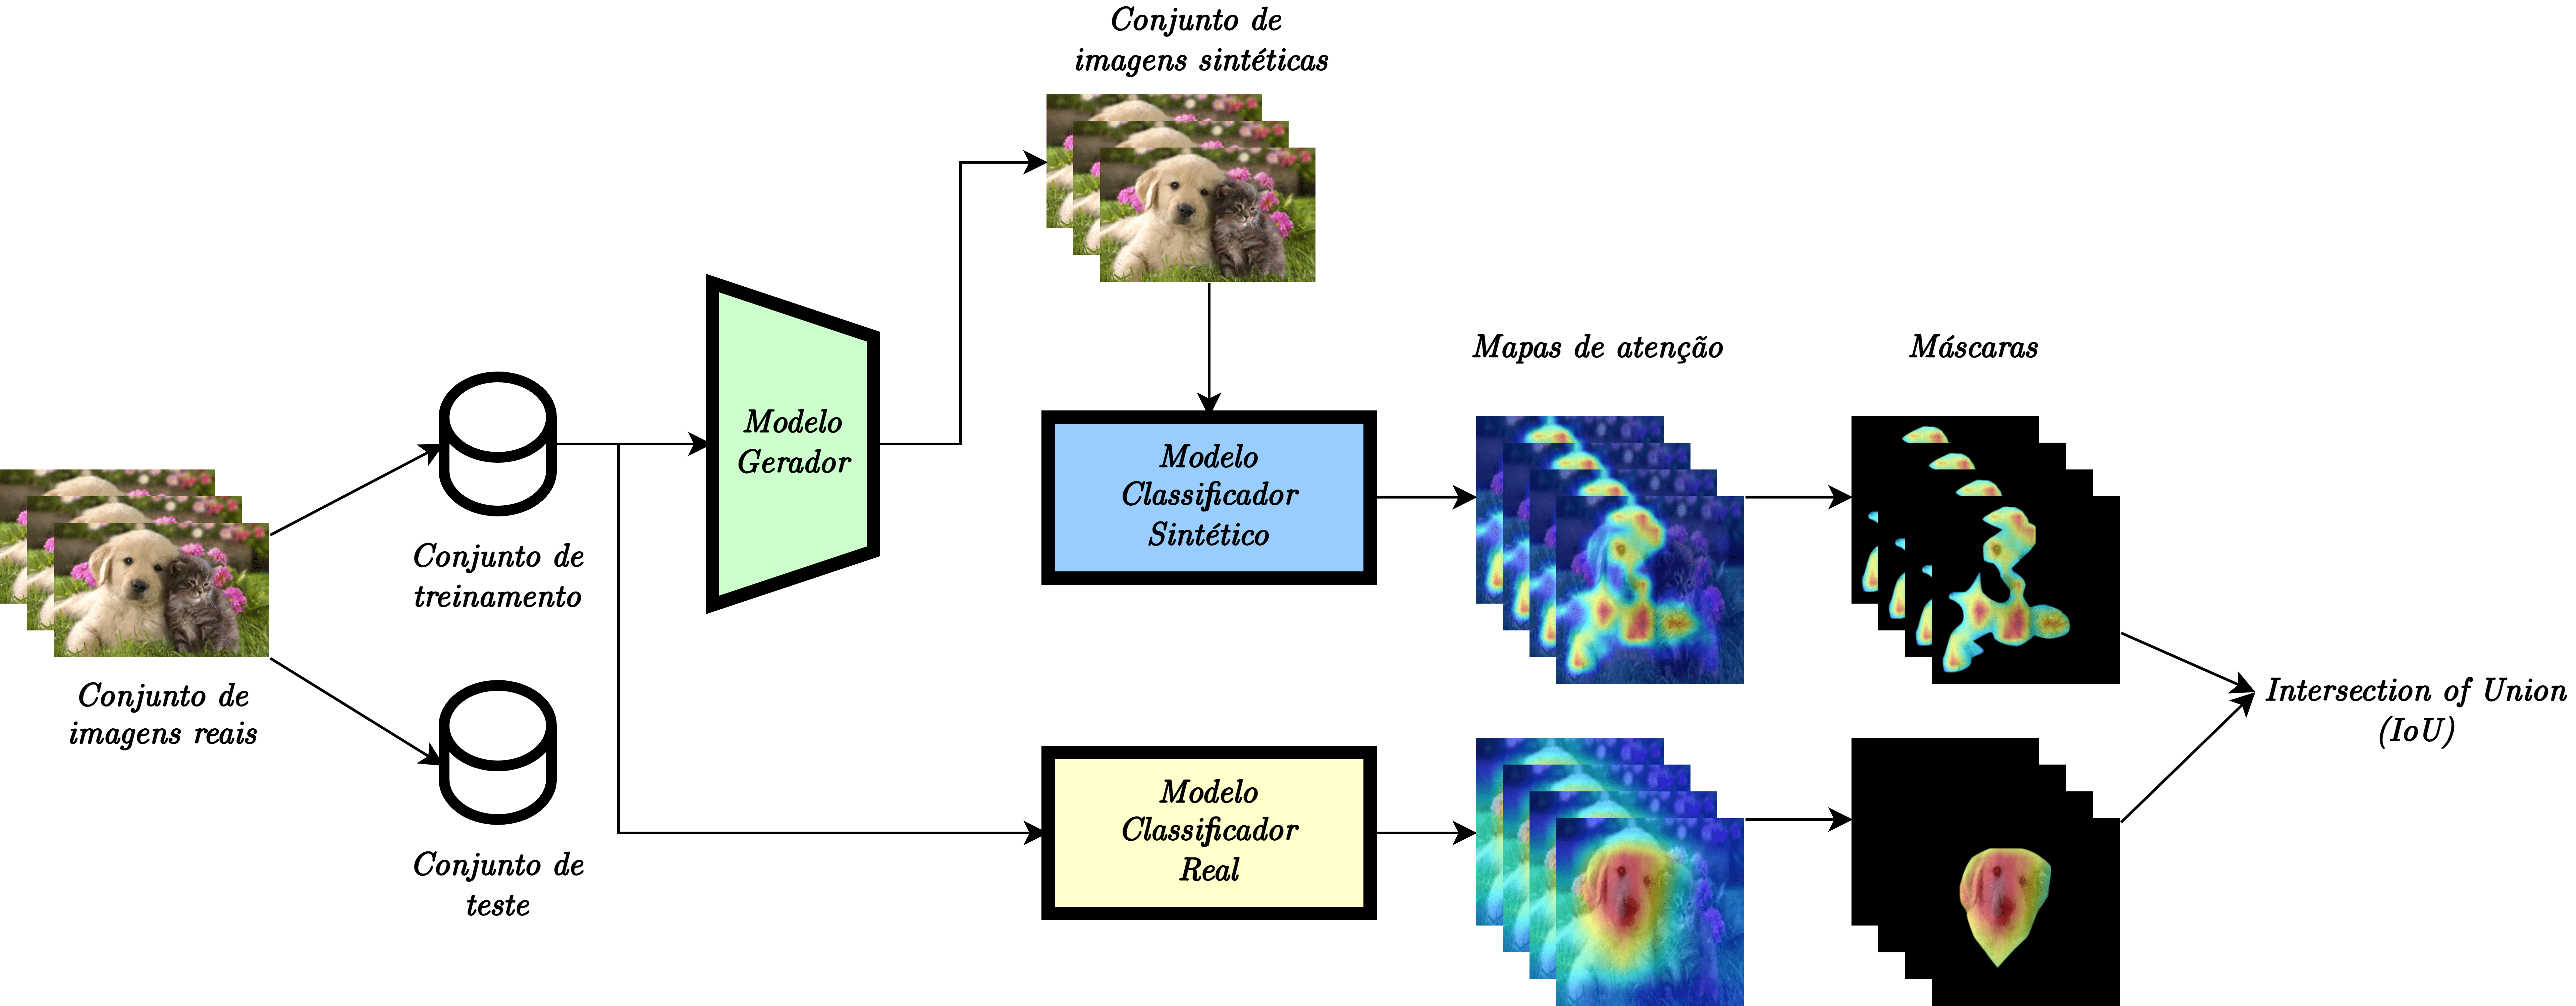
\includegraphics[scale=.65]{imagens/arcabouco.png}
	\label{fig:arcabouco}
  \source{Alexandre Farias, 2024}
\end{figure}

Os modelos classificadores serão treinados ao menos em dois cenários específicos, no primeiro cenário (a) considerando apenas imagens reais e no segundo cenário (b) considerando apenas imagens sintéticas. Na etapa de treinamento, um conjunto de validação será derivado do respectivo conjunto de treinamento para evitar o sobre-ajuste dos modelos e definir critérios de parada antecipada.

\subsubsection{Avaliação}

Utilizando o conjunto de teste os modelos serão submetidos a uma avaliação clássica utilizando as principais métricas encontradas na literatura, como acurácia, precisão, sensibilidade, especificidade e F1.

Juntamente da avaliação de eficácia de aprendizado de máquina, mapas de atenção serão gerados para ambos os modelos em todas as imagens do conjunto de testes utilizando a técnica Grad-CAM++. Com base nos mapas de atenção, técnicas de processamento de imagens serão utilizadas para produzir máscaras que serão posteriormente empregadas para o cálculo da métrica \textit{Intersection of Union} (IoU) que auxiliará na avaliação da similaridade das características aprendidas pelos diferentes modelos.

\subsubsection{Conjuntos de dados}

Para aplicar a metodologia proposta serão utilizados os conjuntos de dados \textit{Chest X-Ray Images (Pneumonia)}\footnote{https://www.kaggle.com/datasets/paultimothymooney/chest-xray-pneumonia?resource=download} e CIFAR-10\footnote{https://www.cs.toronto.edu/~kriz/cifar.html}. O Primeiro conjunto de dados contem imagens de raio-x de tórax de pulmões saudáveis e não saudáveis, o problema de aprendizado a ser resolvido será a classificação binária. Já o segundo conjunto de dados, contêm imagens de várias classes distintas, como aviões, automóveis, cães, gatos, navios e outros animais, para este conjunto de dados o objetivo será o desenvolvimento de um classificador multi-classe.
Além da notável diferença na natureza dos conjuntos de dados, a escolha dos conjuntos se dá também pela diferença de diversidade das amostras, permitindo avaliar os modelos de geração e classificação em conjuntos de menor e maior nível de variação entre as instâncias.

\section{Contribuições}
O desenvolvimento deste projeto contribui para o avanço na metodologia de desenvolvimento e avaliação de modelos de geração de imagens e modelos de classificação treinados em conjuntos de dados sintéticos. Especificamente serão produtos deste trabalho:

\begin{enumerate}
    \item Método de avaliação padronizado contemplando o padrão-ouro atual e novas medidas de interpretabilidade relevantes para detectar problemas de sub-especificação.
    \item Biblioteca \textit{open source} na linguagem de programação Python com o método proposto implementado.
\end{enumerate}


\section{Escopo}

O escopo desta pesquisa se limita a avaliação de modelos de classificação treinados em conjuntos de imagens sintéticas geradas por GANs e \textit{diffusion models}. O presente projeto não inclui a avaliação da qualidade de séries temporais, conjuntos de dados relacionais ou dados tabulares sintéticos. Os métodos de geração e avaliação envolvidos neste trabalho não se aplicam a dados tabulares estruturados.


\bibliography{referencias/referencias}

\end{document}
